% 1983 年全国卷（文科）第 11 题：直角三角形板 ABC 的 BC 边在平面 α 内，A 在 α 内的射影为 N；连 AB、AC、AN、NB、NC、BC，其中 NC 及 α 后边被面 ANC 遮住的一段画虚线（按源卷布局）
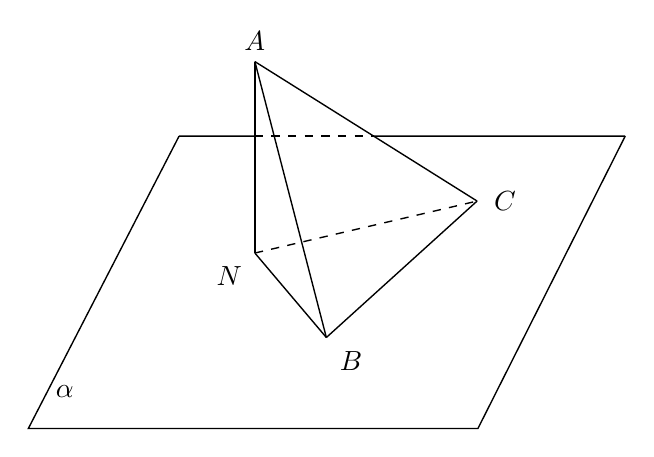
\begin{tikzpicture}[scale=1.1, line width=0.5pt,
  every node/.style={inner sep=1.5pt}]
  % 平面 α 的平行四边形（后边 TL—TR 中段被遮挡，画虚线）
  \coordinate (TL) at (0.90,3.25);
  \coordinate (TR) at (6.05,3.25);
  \coordinate (BR) at (4.35,-0.125);
  \coordinate (BL) at (-0.84,-0.125);
  \draw (TR) -- (BR) -- (BL) -- (TL);
  \draw (TL) -- (1.775,3.25);
  \draw[dashed] (1.775,3.25) -- (3.145,3.25);
  \draw (3.145,3.25) -- (TR);
  % 顶点
  \coordinate (A) at (1.775,4.11);
  \coordinate (N) at (1.775,1.90);
  \coordinate (C) at (4.34,2.50);
  \coordinate (B) at (2.60,0.925);
  % 棱
  \draw (A) -- (N);
  \draw (A) -- (B);
  \draw (A) -- (C);
  \draw (N) -- (B);
  \draw (B) -- (C);
  \draw[dashed] (N) -- (C);
  % 标注
  \node[anchor=south] at (1.775,4.18) {$A$};
  \node[anchor=north east] at (1.68,1.80) {$N$};
  \node[anchor=west] at (4.48,2.50) {$C$};
  \node[anchor=north west] at (2.70,0.82) {$B$};
  \node at (-0.42,0.30) {$\alpha$};
\end{tikzpicture}
